\documentclass[10pt,twocolumn,letterpaper]{article}

\usepackage{cvpr}
\usepackage{times}
\usepackage{epsfig}
\usepackage{graphicx}
\usepackage{amsmath}
\usepackage{amssymb}
\usepackage{caption}
\usepackage{subcaption}
\usepackage{booktabs}
\usepackage{makecell}

% Include other packages here, before hyperref.

% If you comment hyperref and then uncomment it, you should delete
% egpaper.aux before re-running latex.  (Or just hit 'q' on the first latex
% run, let it finish, and you should be clear).
\usepackage[pagebackref=true,breaklinks=true,letterpaper=true,colorlinks,bookmarks=false]{hyperref}

%%%%%%%%% PAPER ID  - PLEASE UPDATE
\def\cvprPaperID{0947} % *** Enter the CVPR Paper ID here
\def\httilde{\mbox{\tt\raisebox{-.5ex}{\symbol{126}}}}

\begin{document}

%%%%%%%%% TITLE - PLEASE UPDATE
\title{Guided Proofreading of Automatic Segmentations for Connectomics}  % **** Enter the paper title here

\maketitle
\thispagestyle{empty}

Thank you for your constructive comments. We will fix all minor issues. We would like to clarify the following major remarks.

\section{Quantitative Evaluation}
Reviewer 2 requests an objective quantitative evaluation. We define such experiments in line 573-590 and report the results in Fig.~6, Fig.~7 and line 792-818 (also in supplemental Sec.~2 and 3). The evaluation is fully numeric and we report VI scores. We will change the wording in the manuscript to make this more clear.

\section{Reproducibility}
Reviewer 2 expresses concerns regarding reproducibility. However, we define all parameters in the manuscript and promise to release code and data (line 847).

\section{Optimal Parameters}
Reviewer 2 


\section{Training Data Sets U-net vs. GP}
Reviewer 3 raises the question if GP was trained on the same data as membrane detection (U-net). There was no overlap in training the classifiers (Tab.~\ref{tab:trainingdata}).

\begin{table}[h]
\caption{Training data of membrane detection vs. taining data of GP (for supplemental material).}%While the training of our classifier is more expensive, testing accuracy is superior. }
\resizebox{\linewidth}{!}{
\begin{tabular}{lrrrr}
\toprule
Dataset & \makecell{Training Set\\Membrane Detection (U-Net)} & \makecell{Training Set\\Guided Proofreading} \\ 
\midrule
\makecell{\emph{L. Cylinder}\\~} & \makecell{AC3+AC4\\($1024\times1024\times175$vx)} & \makecell{L. Cylinder\\($2048\times2048\times250$vx)} \\ 
\makecell{\emph{AC4 subvolume}\\~} & \makecell{AC4 excl. test\\ ($1024\times1024\times90$vx)} &  \makecell{L. Cylinder\\ ($2048\times2048\times250$vx)} \\ 
\makecell{\emph{CREMI A/B/C}\\~} & \makecell{AC3+AC4\\($1024\times1024\times175$vx)} & \makecell{CREMI A/B/C\\($1250\times1250\times300$vx)} \\ 
\bottomrule
\end{tabular} 
}
\label{tab:trainingdata}
\end{table}


\section{Faster Correction Times}
There seems to be a misunderstanding 


\section{Merge Error Detection}

\begin{figure}[h]
\centering
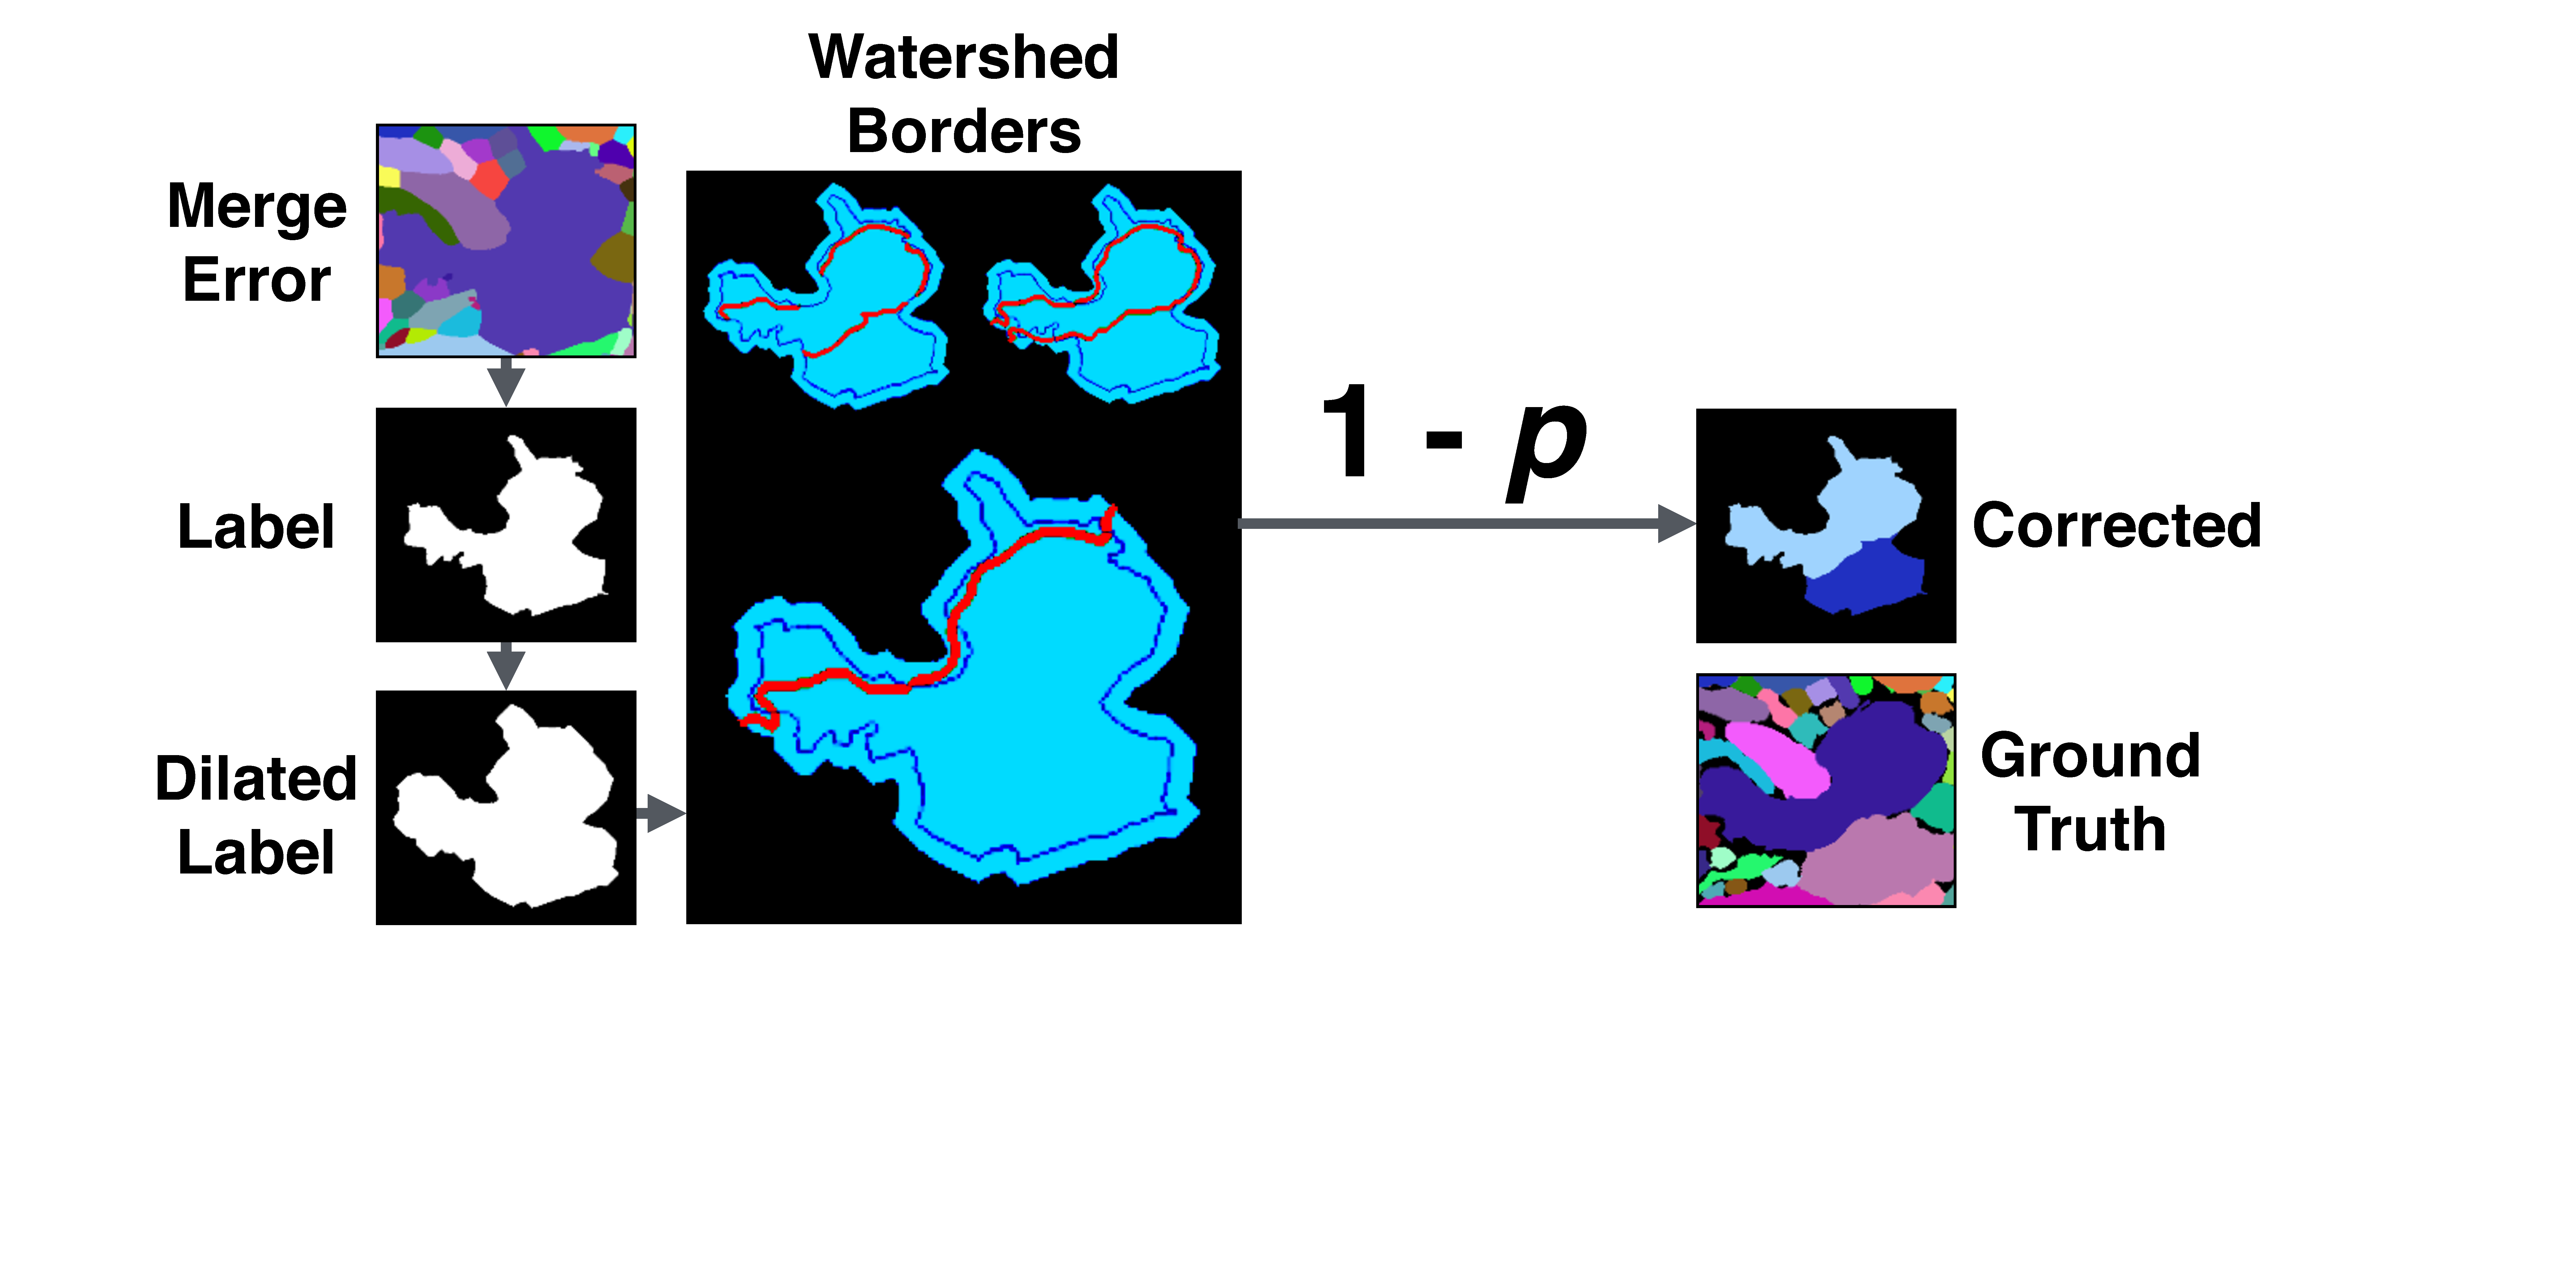
\includegraphics[width=\linewidth]{gfx/merge_error_v4.pdf}
\caption{Updated Figure 4. (not yet)}
\label{fig:merge_error}
\end{figure}


\section{}


{\small
\bibliographystyle{ieee}
\bibliography{egbib}
}

\end{document}
